\documentclass[Ligatures=TeX,table,brazil,svgnames,usetotalslideindicator,comp
ress,10pt]{beamer}

\usetheme[titleformat=allsmallcaps]{metropolis}

\usepackage{polyglossia}
\setdefaultlanguage{brazil}
\disablehyphenation

\usepackage[cachedir=/tmp/minted-\jobname]{minted}
\usemintedstyle{pastie}

\usepackage{graphicx}
\graphicspath{{./figuras/}}

%\usepackage{textpos}

%\usepackage{xspace}
%\usepackage{mdwlist}
%\usepackage{siunitx}
\usepackage{alltt}
\usepackage{multicol}
\usepackage{multirow}
%\usepackage{amsmath}

\usepackage{cancel}
%\usepackage[simplified]{pgf-umlcd}
%\usepackage{pgf-umlsd}

\usepackage{smartdiagram}

\newcommand{\setcoverbg}{
    \setbeamertemplate{background}
     {
\includegraphics[width=\paperwidth,height=\paperheight]{backgrounds/coverbg}}
}
\newcommand{\setintersectionbg}{
    \setbeamertemplate{background}
     {
\includegraphics[width=\paperwidth,height=\paperheight]{backgrounds/blank}}
}
\newcommand{\setsectionbg}{
    \setbeamertemplate{background}
     {
\includegraphics[width=\paperwidth,height=\paperheight]{backgrounds/slidebg2}}
}


\title{REST - Uma Breve Introdução}

\subtitle{MCTA025-13 - Sistemas Distribuídos}

\author{Emilio Francesquini e Fernando Teubl}
\institute{Centro de Matemática, Computação e Cognição\\ Universidade Federal do ABC}
\date{25 de julho de 2018}

\begin{document}

\setcoverbg
\maketitle

\setsectionbg

\begin{frame}
  \frametitle{Disclaimer}
  \begin{itemize}
  \item Estes slides foram preparados para o curso de \textbf{Sistemas
      Distribuídos na UFABC}.
  \item Este material pode ser usado livremente desde que sejam
    mantidos, além deste aviso, os créditos aos autores e
    instituições.
  \item Estes slides foram adaptados com base no material disponível
    em
    \begin{itemize}
      \item A Brief Introduction to REST - \url{http://www.infoq.com/articles/rest-introduction}
      \item JSR 311: JAX-RS: The Java API for RESTful Web Services - \url{https://jcp.org/en/jsr/detail?id=311}
      \item Jersey - RESTful Web Services in Java - \url{https://jersey.github.io}
      \item Putting Java to REST - \url{http://java.dzone.com/articles/putting-java-rest}
      \item REST Tutorial - \url{https://www.devmedia.com.br/rest-tutorial/28912}
    \end{itemize}
  \end{itemize}
\end{frame}

\begin{frame}
  \frametitle{REST}
  \begin{itemize}
  \item \textbf{RE}presentational \textbf{S}tate \textbf{T}ransfer
  \item Serviços que seguem essa linha são comumente chamados de
    RESTful
  \item Modelo apresentado na tese de doutoramento de
    Roy T. Fielding (UC Irvine, 2000)
  \end{itemize}
\end{frame}


\begin{frame}
  \frametitle{REST - Princípios}
  \begin{itemize}
  \item Atribuição de identificadores
  \item Associação de recursos
  \item Utilização de métodos padrão
  \item Multiplicidade de representações
  \item Comunicação sem manutenção de estado
  \end{itemize}
\end{frame}

\begin{frame}
  \frametitle{Identificadores}
  \begin{itemize}
  \item Todas as abstrações do sistema merecem ser
    identificadas
  \item Não apenas uma abstração individualmente deve
    ser identificada, mas qualquer conjunto destas
    abstrações que faça sentido também pode ser
    identificado por um id. Por exemplo:
    \begin{itemize}
    \item Todas as latas de ervilha
    \item Todas as pessoas que tem endereço em SP
    \end{itemize}
  \end{itemize}
\end{frame}

\begin{frame}
  \frametitle{Identificadores e a Web}
  \begin{itemize}
  \item Na web, o jeito mais natural de fazer tal identificação é através de URIs
    \begin{itemize}
    \item \texttt{http://example.com/customers/1234}
    \item \texttt{http://example.com/orders/2007/10/776654}
    \item \texttt{http://example.com/orders/2007/11}
    \item \texttt{http://example.com/products?color=green}
    \end{itemize}
  \item Sem paúra!
    \begin{itemize}
    \item Anos de prática OO nos ensinaram a não expor os detalhes de implementação, ainda mais ids
      do BD
    \item A idéia toda é a de que os conceitos (recursos) que você desejará expor são geralmente
      muito mais abrangentes do que uma linha no BD
    \end{itemize}
  \end{itemize}
\end{frame}


\begin{frame}[fragile]
  \frametitle{Associação - HATEOAS}
  \begin{itemize}
  \item \alert{HATEOAS} - Hypermedia As The Engine Of Application State
  \item Significa que tudo deve ser ligado. Considere o seguinte exemplo de uma resposta a
    uma requisição de pesquisa por pedidos
  \end{itemize}

\begin{minted}{xml}
  <pedido ref='http://xyz.com/pedido/1234'>
    <qtd>23</qtd>
    <produto ref='http://abc.com/produtos/4554'/>
    <cliente ref='http://jkl.com/clientes/7654'/>
  </pedido>
\end{minted}
\end{frame}



\begin{frame}[fragile]
  \frametitle{Métodos de Acesso Padronizados}

  Pode-se imaginar que todo recurso é algo
  semelhante a:

\begin{minted}{java}
class Resource {
 Resource(URI u);
 Response get();
 Response post(Request r);
 Response put(Request r);
 Response delete();
}
\end{minted}
  Onde:
  \begin{itemize}
  \item \alert{GET} – Pega uma representação do recurso
  \item \alert{PUT} – Cria ou atualiza, se já existir o
    recurso, com as informações passadas
  \item \alert{DELETE} – Apaga o recurso
  \item \alert{POST} – Única operação \textbf{não idempotente} (ao menos na
    definição original).  Geralmente significa criação de um recurso
    ou ativação de algum processamento arbitrário.
  \end{itemize}
\end{frame}


\begin{frame}
  \frametitle{Métodos de Acesso Padronizados}
  \begin{itemize}
  \item Essas restrições devem ser respeitadas pelos serviços RESTful
    \begin{itemize}
    \item No entanto, na vida real, nem todas essas restrições
      semânticas são respeitadas e é preciso avaliar cada caso de uso
      individualmente
    \end{itemize}
  \item Pode ser difícil imaginar que uma aplicação modelada de uma
    maneira OO possa ser mapeada desta maneira
  \end{itemize}
\end{frame}


\begin{frame}
  \frametitle{Representado um sistema OO}
  \begin{figure}[ht]
    \centering
    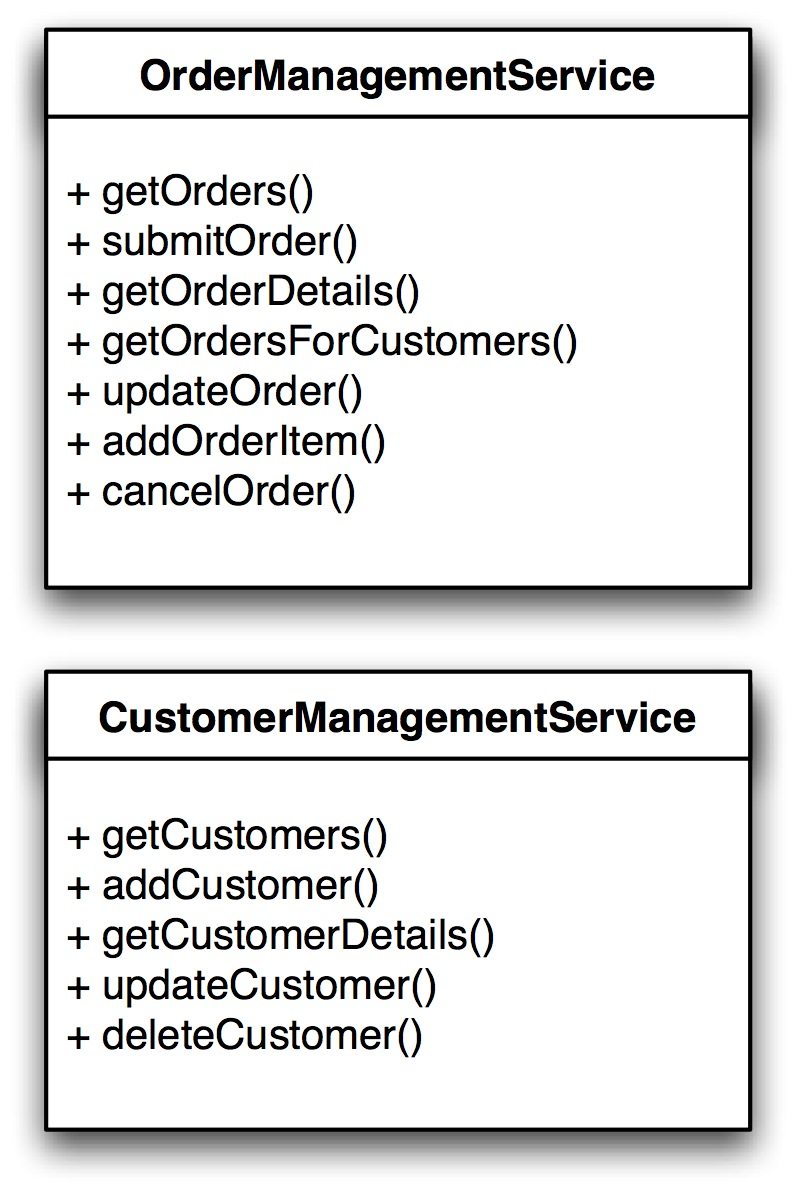
\includegraphics[width=0.5\textwidth]{figuras/rest1.jpg}
    \\\tiny{Figura: Tilkov, 2007}
  \end{figure}
\end{frame}

\begin{frame}
  \frametitle{Representado um sistema OO}
  \begin{figure}[ht]
    \centering
    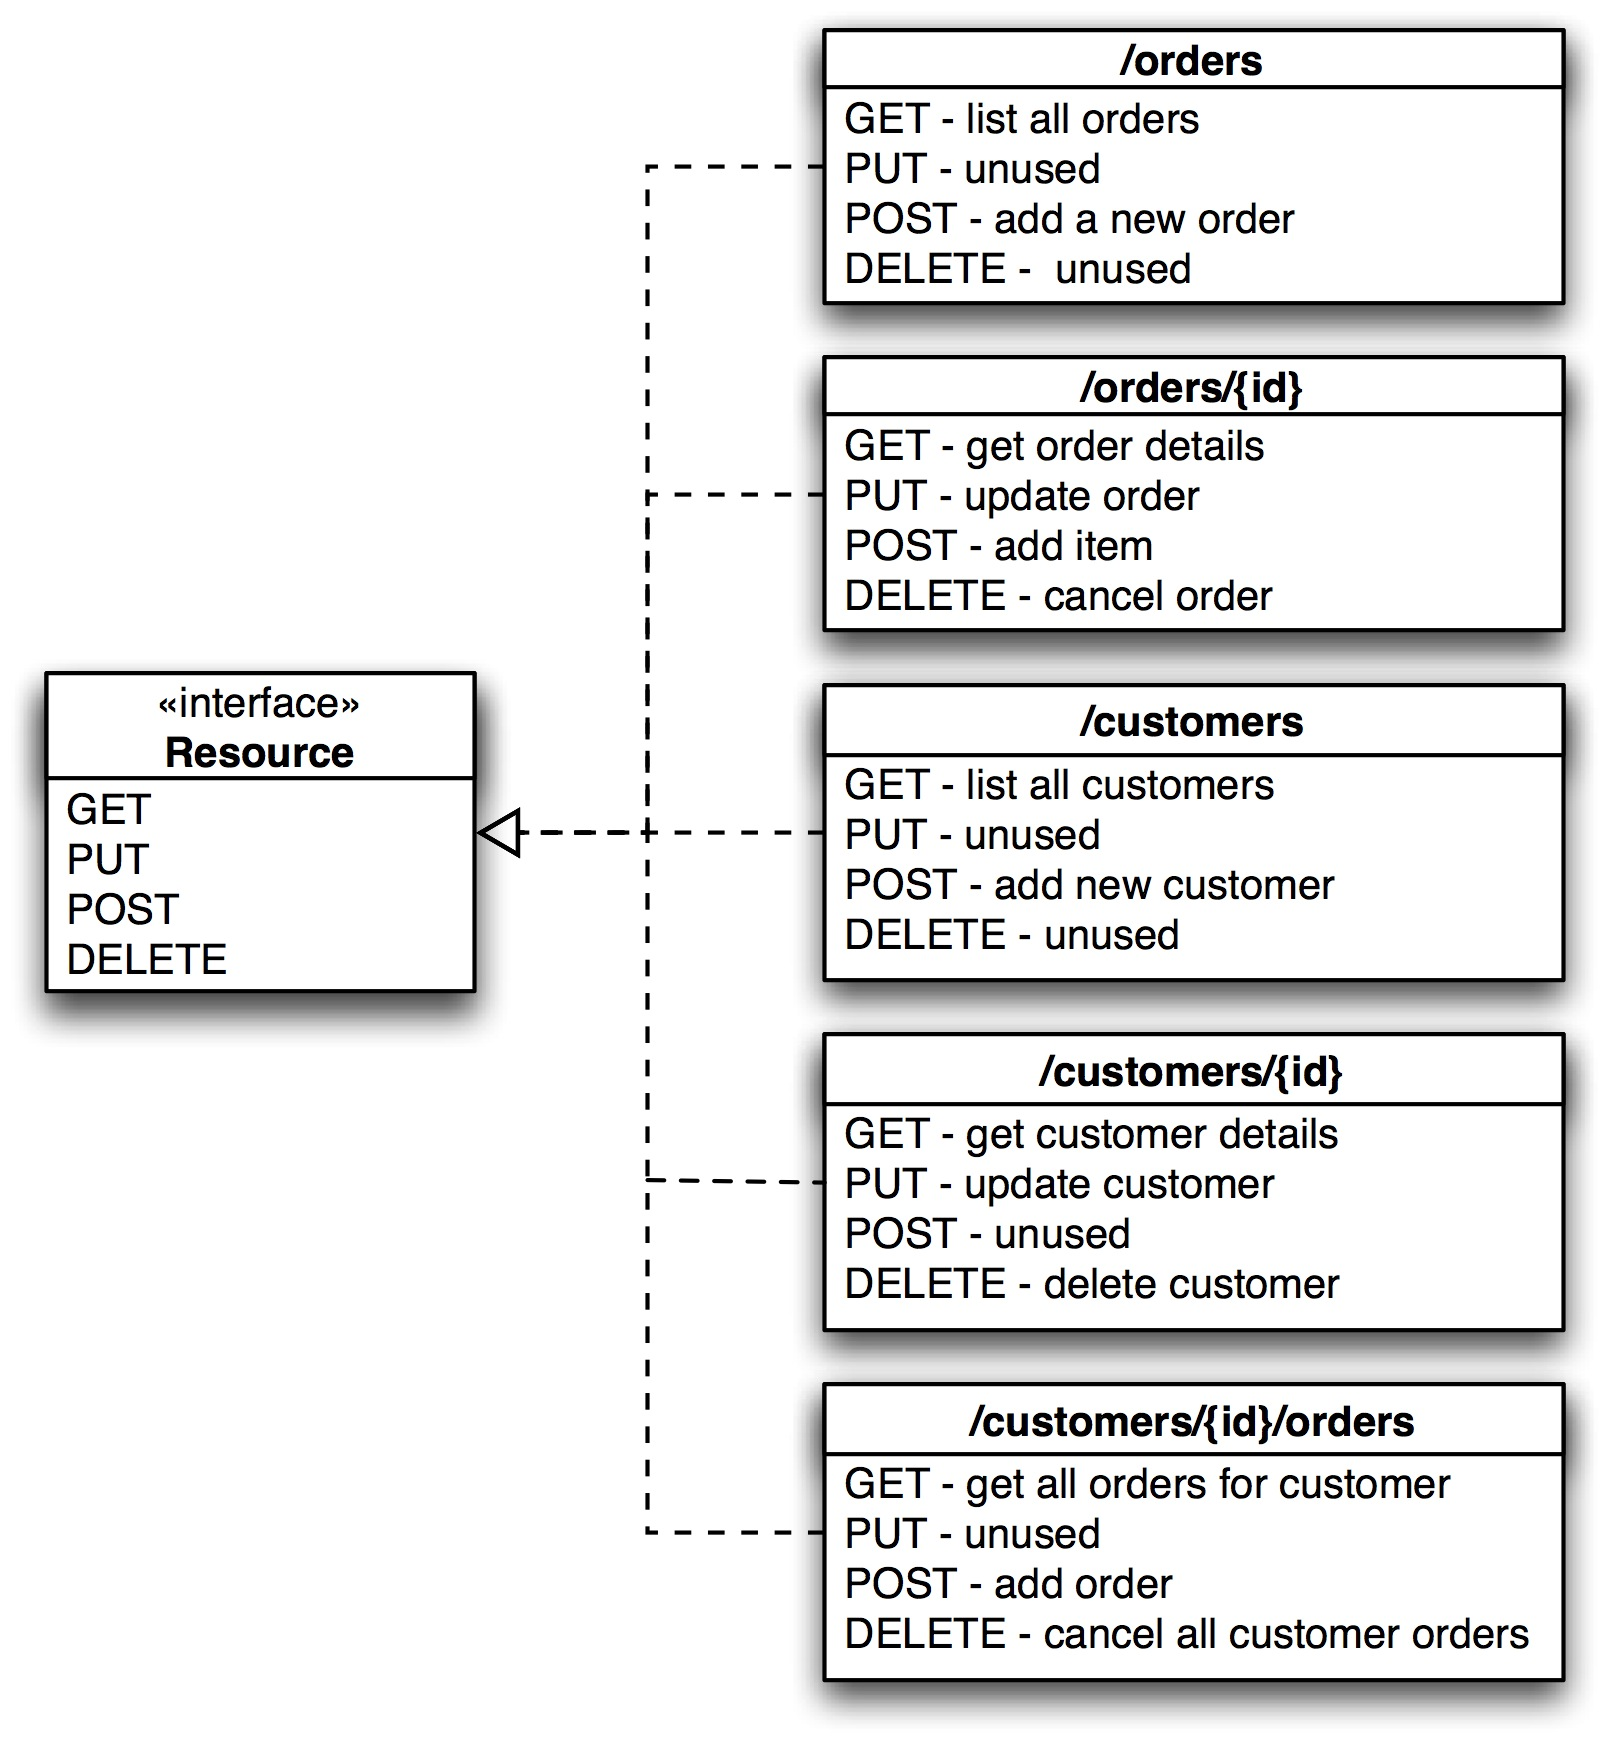
\includegraphics[width=0.7\textwidth]{figuras/rest2.jpg}
    \tiny{Figura: Tilkov, 2007}
  \end{figure}
\end{frame}

\begin{frame}
  \frametitle{Múltiplas Representações}

  \texttt{\mbox{}\\
    GET /clientes/1234 HTTP/1.1\\
    Host: xyz.com\\
    Accept: application/meucliente+xml\\
    GET /clientes/1234 HTTP/1.1\\
    Host: xyz.com\\
    Accept: text/x-vcard\\
  }

  \begin{itemize}
  \item \textbf{Possível uso:} uma mesma API que gera as informações em HTML
    para uma página ou em um formato XML para ser usada por alguma
    aplicação
  \end{itemize}
\end{frame}


\begin{frame}
  \frametitle{Comunicação sem Manutenção de Estado}

  \begin{itemize}
  \item Depois de ver os princípios anteriores, fica claro como fazer isso
  \item Atenção: Colocar na URI um ID de sessão não transforma seu web service em um RESTful
  \item Vantagens
    \begin{itemize}
    \item Diminuição da carga do servidor
    \item Escalabilidade
    \item Independência da implementação do servidor
    \item Independência entre servidores
    \end{itemize}
  \end{itemize}

\end{frame}

\begin{frame}
  \frametitle{HTTP RESTful}
  \begin{itemize}
  \item Também tem sido chamado de WebAPI
  \item Muito usado para fazer mashups
  \item Um dos pilares para as páginas de conteúdo mais modernas
  \item Faz a junção das informações direto no cliente e não mais no servidor
  \end{itemize}
\end{frame}

\begin{frame}
  \frametitle{REST}
  \begin{itemize}
  \item A especificação propriamente dita não diz nada quanto a HTTP
  \item Também não especifica o número de operações, apenas determina
    que a interface deve ser padrão
  \item Não é demais supor que REST e HTTP tenham se influenciado
    mutuamente já que o Fielding, criador e descritor do REST também
    tenha definido muitos dos padrões HTTP
  \end{itemize}
\end{frame}

\begin{frame}
  \frametitle{Exemplos}
  Praticamente todos os grandes sites da Internet tem APIs REST.
  \begin{itemize}
  \item Twitter
  \item Flickr
  \item Google
  \item Amazon
  \item Facebook
  \item \ldots
  \end{itemize}
\end{frame}

\begin{frame}
  \frametitle{REST - Implementação em JAVA}
  \alert{\textbf{JAX-RS}}
  \begin{itemize}
  \item Criado para facilitar a implementação de serviços REST em Java
  \item Baseado em anotações
  \item Evita a tarefa um tanto entediante de fazer o processamento de
    URIs, XMLs, ...
  \end{itemize}
\end{frame}

\begin{frame}[fragile]
  \frametitle{REST - JAX-RS - Serviço Simples}

\begin{minted}{java}
  @Path("/orders")
  public class OrderEntryService {
    @GET
    public String getOrders() {...}
  }
\end{minted}

\begin{itemize}
\item Responde por requisições \alert{\texttt{GET}} no endereço:
  \begin{itemize}
  \item \url{http://exemplo.com/orders}
  \end{itemize}
\end{itemize}
\end{frame}


\begin{frame}[fragile]
  \frametitle{REST - JAX-RS - Lendo os Parâmetros}

\begin{minted}{java}
  @Path("/orders")
  public class OrderEntryService {
    @GET
    public String getOrders(@QueryParam("size")
                            @DefaultValue("50")
                            int size) {
      ...
    }
  }
\end{minted}

\begin{itemize}
\item Responde por requisições \alert{\texttt{GET}} no endereço:
  \begin{itemize}
  \item \texttt{http://exemplo.com/orders?\alert{size=30}}
  \end{itemize}
\end{itemize}
\end{frame}

\begin{frame}[fragile]
  \frametitle{REST - JAX-RS - Composição de Endereços}

\begin{minted}{java}
  @Path("/orders")
  public class OrderEntryService {
    @GET
    @Path{"/{id}"}
    public String getOrder(@PathParam("id")
                           int orderId){
      ...
    }
  }
\end{minted}

\begin{itemize}
\item Responde por requisições \alert{\texttt{GET}} no endereço:
  \begin{itemize}
  \item \texttt{http://exemplo.com/orders/\alert{3333}}
  \end{itemize}
\item Mas não no endereço:
  \begin{itemize}
  \item \texttt{http://exemplo.com/orders/3333/entries}
  \end{itemize}
\item Há também a possíbilidade de se usar expressões regulares:
  \begin{minted}{java}
@Path("{id: \\d+}")
  \end{minted}
\end{itemize}
\end{frame}


\begin{frame}[fragile]
  \frametitle{REST - JAX-RS - Content Type}

\begin{minted}{java}
  @Path("/orders")
  public class OrderEntryService {
    @GET
    @Path("{id}")
    @Produces("application/xml")
    public String getOrder(@PathParam("id")
                            int orderId) {
      ...
    }
  }
\end{minted}

\begin{itemize}
\item Só será chamado caso o cliente envie no pedido que ele aceita \texttt{application/xml}
\item O Firefox, por exemplo, envia como tipos aceitos:\\
\end{itemize}
    \footnotesize{\texttt{Accept: text/html,application/xhtml+xml,application/xml;q=0.9,*/*;q=0.8}}

\end{frame}


\begin{frame}[fragile]
  \frametitle{REST - JAX-RS - Negociação de Conteúdo}

{\footnotesize
\begin{minted}{java}
  @Path("/orders")
  public class OrderEntryService {
    @GET
    @Path("{id}")
    @Produces("application/xml")
    public String getOrder(@PathParam("id") int orderId) {...}

    @GET
    @Path("{id}")
    @Produces("text/html")
    public String getOrderHtml(@PathParam("id") int orderId) {...}

    @GET
    @Path("{id}")
    @Produces("application/json")
    public String getOrderJson(@PathParam("id") int orderId) {...}

  }
\end{minted}
}

\end{frame}

\begin{frame}[fragile]
  \frametitle{REST - JAX-RS - Codificação de Conteúdo}
  \begin{itemize}
  \item Em vez de fazermos o empacotamento (\emph{marshalling}) de
    conteúdo manualmente (note o tipo de retorno sendo \texttt{String}
    nos exemplos), podemos fazer automaticamente
  \end{itemize}
\end{frame}

\begin{frame}[fragile]
  \frametitle{REST - JAX-RS - Codificação de Conteúdo}

{\footnotesize
\begin{minted}{java}
  @Path("/orders")
  public class OrderEntryService {
    @GET
    @Path("{id}")
    @Produces("application/xml")
    public Order getOrder(@PathParam("id") int orderId) {...}
    ...
  }
  @XmlRootElement(name="order")
  public class Order {
    @XmlElement(name="id")
    int id;
    @XmlElement(name="order-entries")
    List<OderEntry> entries;
    ...
  }
\end{minted}
}

  \begin{itemize}
  \item O empacotamento também pode ser feito automaticamente caso a
    classe do objeto devolvido como retorno obedeça as regras de um
    \emph{bean}, o seja, tenha definido os \emph{getters} e
    \emph{setters}.
  \end{itemize}
\end{frame}


\begin{frame}
  \frametitle{Exemplo - Criação de uma Agenda}
  \begin{itemize}
  \item Vamos criar uma agenda que guarda
    \begin{itemize}
    \item Nomes
    \item Emails
    \item Telefones
    \end{itemize}
  \item A linguagem será Java utilizando Jersey
  \end{itemize}

\end{frame}

\begin{frame}[fragile]
  \frametitle{Preparando o ambiente}
  \begin{itemize}
  \item Para criar um projeto Maven básico com tudo o que precisamos execute a seguinte linha de comando em um terminal:
  \end{itemize}
{\footnotesize \texttt{
    \$ mvn archetype:generate \textbackslash \\
    \mbox{ }\mbox{ }-DarchetypeArtifactId=jersey-quickstart-grizzly2 \textbackslash \\
    \mbox{ }\mbox{ }-DarchetypeGroupId=org.glassfish.jersey.archetypes \textbackslash \\
    \mbox{ }\mbox{ }-DinteractiveMode=false -DgroupId=sd \textbackslash \\
    \mbox{ }\mbox{ }-DartifactId=servico-agenda -Dpackage=sd \textbackslash \\
    \mbox{ }\mbox{ }-DarchetypeVersion=2.27
}}

\begin{itemize}
\item Caso receba um erro que o mvn não foi encontrado, instale-o
  fazendo \texttt{sudo apt-get install maven}
\end{itemize}

\end{frame}

\begin{frame}[fragile]
  \frametitle{Configurando o projeto}
  \begin{itemize}
  \item Edite o arquivo \texttt{pom.xml} para habilitar o marshalling/unmarshalling automático para Json
    \begin{itemize}
    \item Basta descomentar as linhas indicadas
    \end{itemize}
  \item Altere o arquivo \texttt{Main.java} para que ele passe a escutar na raiz do nosso servidor (pode alterar a porta também caso necessário.
    \begin{itemize}
    \item Basta alterar a linha 16 para que fique como abaixo:
    \end{itemize}
  \end{itemize}
\begin{minted}{java}
public static final String BASE_URI =
  "http://localhost:8080/";
\end{minted}
\end{frame}

\begin{frame}[fragile]
  \frametitle{Executando o projeto}
  \begin{itemize}
  \item O Maven já vai ter criado um serviço simples cuja implementação está em \texttt{MyResource.java}
  \end{itemize}

\begin{minted}{java}
package sd;
import javax.ws.rs.GET;
import javax.ws.rs.Path;
import javax.ws.rs.Produces;
import javax.ws.rs.core.MediaType;

@Path("myresource")
public class MyResource {
    @GET
    @Produces(MediaType.TEXT_PLAIN)
    public String getIt() {
        return "Got it!";
    }
}
\end{minted}

\end{frame}

\begin{frame}[fragile]
  \frametitle{Executando o projeto}
  \begin{itemize}
  \item Para executá-lo, basta rodar na raiz do projeto:
  \end{itemize}

{\footnotesize
\texttt{\$ mvn compile}\\
\texttt{\$ mvn exec:java}
\begin{minted}{bash}
INFO: [HttpServer] Started.
Jersey app started with WADL available at
http://localhost:8080/application.wadl
Hit enter to stop it...
\end{minted}
}
\end{frame}

\begin{frame}[fragile]
  \frametitle{Executando o projeto}
Conteúdo de \texttt{http://localhost:8080/application.wadl}

{\footnotesize
\begin{minted}{xml}
  <application xmlns="http://wadl.dev.java.net/2009/02">
  ...
  <grammars/>
    <resources base="http://localhost:8080/">
      <resource path="myresource">
        <method id="getIt" name="GET">
          <response>
            <representation mediaType="text/plain"/>
          </response>
        </method>
      </resource>
    </resources>
  </application>
\end{minted}
}
\end{frame}

\begin{frame}[fragile]
  \frametitle{Agenda - Implementação}
  A classe Email
  \begin{minted}{java}
package sd;
public class Email {
    private String tipo;
    private String endereco;
    public Email() {}
    public Email(String tipo, String endereco) {
        this.tipo = tipo;
        this.endereco = endereco;
    }
    public String getTipo() {...}
    public void setTipo(String tipo) {...}
    public String getEndereco() {...}
    public void setEndereco(String endereco) {...}
    public String toString() {...}
}
  \end{minted}

\end{frame}


\begin{frame}[fragile]
  \frametitle{Agenda - Implementação}
  A classe Telefone
  \begin{minted}{java}
package sd;
public class Telefone {
    private String tipo;
    private String numero;
    public Telefone() {}
    public Telefone(String tipo, String numero) {
        this.tipo = tipo;
        this.numero = numero;
    }
    public String getTipo() {...}
    public void setTipo(String tipo) {...}
    public String getNumero() {...}
    public void setNumero(String numero) {...}
    public String toString() {...}
}
\end{minted}

\end{frame}

\begin{frame}[fragile]
  \frametitle{Agenda - Implementação}
  A classe Contato
{\footnotesize
\begin{minted}{java}
package sd;
...
public class Contato {
    private int id;
    private String nome;
    private List<Telefone> telefones = new ArrayList<Telefone>();
    private List<Email> emails = new ArrayList<Email>();

    public int getId() {...}
    public String getNome() {...}
    public List<Telefone> getTelefones() {...}
    public List<Email> getEmails() {...}
    public void setId(int id) {...}
    public void setNome(String nome) {...}
    public void setTelefones(List<Telefone> telefones) {...}
    public void setEmails(List<Email> emails) {...}
    ...
}
\end{minted}
}
\end{frame}


\begin{frame}[fragile]
  \frametitle{Agenda - Implementação}
  A classe \texttt{ServicoContatos}
{\footnotesize
\begin{minted}{java}
package sd;
...
@Path("contatos")
public class ServicoContatos {
  private static Map<Integer, Contato> contatos =
    new HashMap<Integer, Contato>();
  private static int proximoId = 1;
  private void criaContato(String nome,
                           String emailTipo, String email,
                           String telTipo, String tel) {
    int id = proximoId++;
    Contato contato = new Contato();
    contato.setId(id);
    contato.setNome(nome);
    contato.getEmails().add(new Email(emailTipo, email));
    contato.getTelefones().add(new Telefone(telTipo, tel));
    contatos.put(id, contato);
  }
  ...
\end{minted}
}
\end{frame}

\begin{frame}[fragile]
  \frametitle{Agenda - Implementação}
  A classe \texttt{ServicoContatos}
{\footnotesize
\begin{minted}{java}
  ...
  public ServicoContatos() {
    if (contatos.isEmpty()) {
      criaContato("E. Francesquini",
                  "Profissional", "e.francesquini@ufbac.edu.br",
                  "Comercial", "4996 8327");
      criaContato("F. Ferreira ",
                  "Profissional", "fernando.teubl@ufabc.edu.br",
                  "Residencial", "1234 5678");
    }
  }
  ...
\end{minted}
}
\end{frame}


\begin{frame}[fragile]
  \frametitle{Agenda - Implementação}
  A classe \texttt{ServicoContatos} - \texttt{GET}
{\footnotesize
\begin{minted}{java}
  ...
    @GET
    @Produces(MediaType.TEXT_PLAIN)
    public String listPlain() {
        System.out.println("listPlain");
        StringBuffer ret = new StringBuffer();
        for (Contato contato :contatos.values()) {
            ret.append(contato);
            ret.append("\n");
        }
        return ret.toString();
    }

    @GET
    @Produces(MediaType.APPLICATION_JSON)
    public List<Contato> listJson() {
        System.out.println("listJson");
        return new ArrayList(contatos.values());
    }
  ...
\end{minted}
}
\end{frame}

\begin{frame}[fragile]
  \frametitle{Agenda - Implementação}
  A classe \texttt{ServicoContatos} - \texttt{GET}
{\footnotesize
\begin{minted}{java}
  ...
  @GET
  @Produces(MediaType.APPLICATION_JSON)
  @Path("/{id}")
  public Contato getContato(@PathParam("id") int id) {
      System.out.println("getContato");
      Contato ret = contatos.get(id);
      if (ret == null)
          throw new WebApplicationException(404);
      return ret;
  }
  ...
\end{minted}
}
\end{frame}

\begin{frame}[fragile]
  \frametitle{Agenda - Implementação}
  A classe \texttt{ServicoContatos} - \texttt{GET}
{\footnotesize
\begin{minted}{java}
  ...
  @GET
  @Path("/busca/{nome}")
  @Produces(MediaType.APPLICATION_JSON)
  public List<Contato> findByName(@PathParam("nome") String nome) {
      System.out.println("findByName");
      String lcNome = nome.toLowerCase();
      List<Contato> ret = new ArrayList<Contato>();
      for (Contato contato : contatos.values()) {
          if (contato.getNome() != null
              && contato.getNome().toLowerCase().contains(lcNome)) {
              ret.add(contato);
          }
      }
      return ret;
  }
  ...
\end{minted}
}
\end{frame}

\begin{frame}[fragile]
  \frametitle{Agenda - Implementação}
  A classe \texttt{ServicoContatos} - \texttt{POST}
{\footnotesize
\begin{minted}{java}
...
@POST
@Consumes(MediaType.APPLICATION_JSON)
@Produces(MediaType.APPLICATION_JSON)
public Contato add(Contato contato) {
    System.out.println("add");
    if (contato.getNome() == null ||
        contato.getNome().trim().equals("")) {
        throw new WebApplicationException(Response
                               .status(Response.Status.BAD_REQUEST)
                               .entity("Nome é obrigatorio").build());
    }
    contato.setId(proximoId++);
    contatos.put(contato.getId(), contato);
    return contato;
}
...
\end{minted}
}
\end{frame}

\begin{frame}[fragile]
  \frametitle{Agenda - Implementação}
  A classe \texttt{ServicoContatos} - \texttt{PUT}
{\footnotesize
\begin{minted}{java}
...
@PUT
@Path("/{id}")
@Consumes(MediaType.APPLICATION_JSON)
public Response update(@PathParam("id") int id, Contato contato) {
    System.out.println("update");
    if (id != contato.getId()) {
        throw new WebApplicationException(Response
                              .status(Response.Status.BAD_REQUEST)
                              .entity("O id deve ser igual").build());
    }
    contatos.put(id, contato);
    return Response.ok().build();
}
...
\end{minted}
}
\end{frame}


\begin{frame}[fragile]
  \frametitle{Agenda - Implementação}
  A classe \texttt{ServicoContatos} - \texttt{DELETE}
{\footnotesize
\begin{minted}{java}
...
@DELETE
public Response delete(@QueryParam("id") int id) {
    System.out.println("delete");
    Contato cont = contatos.get(id);
    if (cont == null) {
        System.out.println("Não achou");
        throw new WebApplicationException(404);
    }
    contatos.remove(id);
    return Response.ok().build();
}
...
\end{minted}
}
\end{frame}

\begin{frame}[fragile]
  \frametitle{O WADL}
{\footnotesize
\begin{minted}{xml}
<application xmlns="http://wadl.dev.java.net/2009/02">
...
<resources base="http://localhost:8080/">
  <resource path="contatos">
  <method id="listPlain" name="GET">
  <response> <representation mediaType="text/plain"/>  </response>
  </method>
  <method id="listJson" name="GET">
    <response> <representation mediaType="application/json"/> </response>
  </method>
  <method id="add" name="POST">
    <request>
      <representation mediaType="application/json"/>
    </request>
    <response> <representation mediaType="application/json"/> </response>
  </method>
  ...
\end{minted}
}
\end{frame}

\begin{frame}[fragile]
  \frametitle{Acessando o serviço REST}
  Pode-se acessar diretamente pela linha de comando:
{\footnotesize
  \begin{minted}{bash}
$ curl -H "Accept:text/plain" \
  --request GET http://localhost:8080/contatos/
{ 1, E. Francesquini, [{ Profissional:e.francesquini@ufbac.edu.br }],
  [{ Comercial:9876 5432 }] }
{ 2, F. Ferreira , [{ Profissional:fernando.teubl@ufabc.edu.br }],
  [{ Residencial:1234 5678 }] }
$
$ curl -H "Accept:application/json" \
  --request GET http://localhost:8080/contatos/
[{"emails":[{"endereco":"e.francesquini@ufbac.edu.br",
"tipo":"Profissional"}],"id":1,"nome":"E. Francesquini",
"telefones":[{"numero":"9876 5432","tipo":"Comercial"}]},
{"emails":[{"endereco":"fernando.teubl@ufabc.edu.br",
"tipo":"Profissional"}],"id":2,"nome":"F. Ferreira ",
"telefones":[{"numero":"1234 5678","tipo":"Residencial"}]}]
$
\end{minted}
}
\end{frame}

\begin{frame}[fragile]
  \frametitle{Acessando o serviço REST}
{\footnotesize
  \begin{minted}{bash}
$ curl --request DELETE http://localhost:8080/contatos?id=1
$
$ curl -H "Accept:application/json" \
  --request GET http://localhost:8080/contatos/
[{"emails":[{"endereco":"fernando.teubl@ufabc.edu.br",
"tipo":"Profissional"}],"id":2,"nome":"F. Ferreira ",
"telefones":[{"numero":"1234 5678","tipo":"Residencial"}]}]
$
\end{minted}
}
\end{frame}

\begin{frame}[fragile]
  \frametitle{Acessando o serviço REST}
{\footnotesize
\begin{minted}{bash}
$ curl -H "Content-Type:application/json" \
  --request POST http://localhost:8080/contatos/ \
  -d '{"emails":[{"endereco":"maluco@ufabc.edu.br", \
  "tipo":"Pessoal"}], "id":3, "nome":"Maluco UFABC",\
  "telefones":[{"numero":"99999999","tipo":"Celular"}]}'

{"emails":[{"endereco":"maluco@ufabc.edu.br","tipo":"Pessoal"}],
"id":3,"nome":"Maluco UFABC","telefones":[{"numero":"99999999",
"tipo":"Celular"}]}
$
$ curl -H "Accept: application/json" \
  --request GET http://localhost:8080/contatos/
[{"emails":[{"endereco":"fernando.teubl@ufabc.edu.br",
"tipo":"Profissional"}],"id":2,"nome":"F. Ferreira ",
"telefones":[{"numero":"1234 5678","tipo":"Residencial"}]},
{"emails":[{"endereco":"maluco@ufabc.edu.br","tipo":"Pessoal"}],
"id":3,"nome":"Maluco UFABC","telefones":[{"numero":"99999999",
"tipo":"Celular"}]}]
$
\end{minted}
}
\end{frame}

\begin{frame}[fragile]
  \frametitle{Acesso via Java - Versão na Unha}
{\footnotesize
\begin{minted}{java}
public class ClienteREST {
  public static void main(String[] args) {
    ...
    URL url = new URL("http://localhost:8080/contatos");
    HttpURLConnection conn = (HttpURLConnection) url.openConnection();
    conn.setRequestMethod("GET");
    conn.setRequestProperty("Accept", "application/json");
    if (conn.getResponseCode() != 200) {
      throw new RuntimeException("Failed : HTTP error code : "
        + conn.getResponseCode());
    }
    BufferedReader br = new BufferedReader(new InputStreamReader(
      (conn.getInputStream())));
    String output;
    System.out.println("Output from Server .... \n");
    while ((output = br.readLine()) != null) {
      System.out.println(output);
    }
    conn.disconnect();
    ...
  }
}
\end{minted}
}
\end{frame}


\begin{frame}[fragile]
  \frametitle{Acesso via Java - Versão Simplificada}
{\footnotesize
\begin{minted}{java}
import javax.ws.rs.client.Client;
import javax.ws.rs.client.ClientBuilder;
import javax.ws.rs.client.WebTarget;

public class ClienteREST {
  public static void main(String[] args) {
    Client c = ClientBuilder.newClient();
    WebTarget target = c.target("http://localhost:8080/");
    String responseMsg = target.path("contatos")
      .request().get(String.class);
    System.out.println(resposeMsg);
  }
}
\end{minted}
}

Veja o exemplo de uso no diretório \texttt{src/test/} criado pelo Maven.
\end{frame}

\end{document}
